	La etapa de salida clase G se caracteriza principalmente por el manejo eficiente de potencia debido a que conmuta la tensión de alimentación entre dos niveles según lo requiera la señal de entrada.

	En la figura se muestra un esquema básico de la topología, denominada Clase G alternativa.  Los transistores $Q_1$ y $Q_2$ conforman la etapa interior que opera en clase B, siendo $Q3$ y $Q4$ los \textit{drivers} y $R1$ la resistencia de emisor compartida. 

	\begin{figure}[H]
		\centering
		\scalebox{0.5}{% XCircuit output "salida.tex" for LaTeX input from salida.eps
\def\putbox#1#2#3#4{\makebox[0in][l]{\makebox[#1][l]{}\raisebox{\baselineskip}[0in][0in]{\raisebox{#2}[0in][0in]{\scalebox{#3}{#4}}}}}
\def\rightbox#1{\makebox[0in][r]{#1}}
\def\centbox#1{\makebox[0in]{#1}}
\def\topbox#1{\raisebox{-0.60\baselineskip}[0in][0in]{#1}}
\def\midbox#1{\raisebox{-0.20\baselineskip}[0in][0in]{#1}}
   \scalebox{1}{
   \normalsize
   \parbox{6.61458in}{
   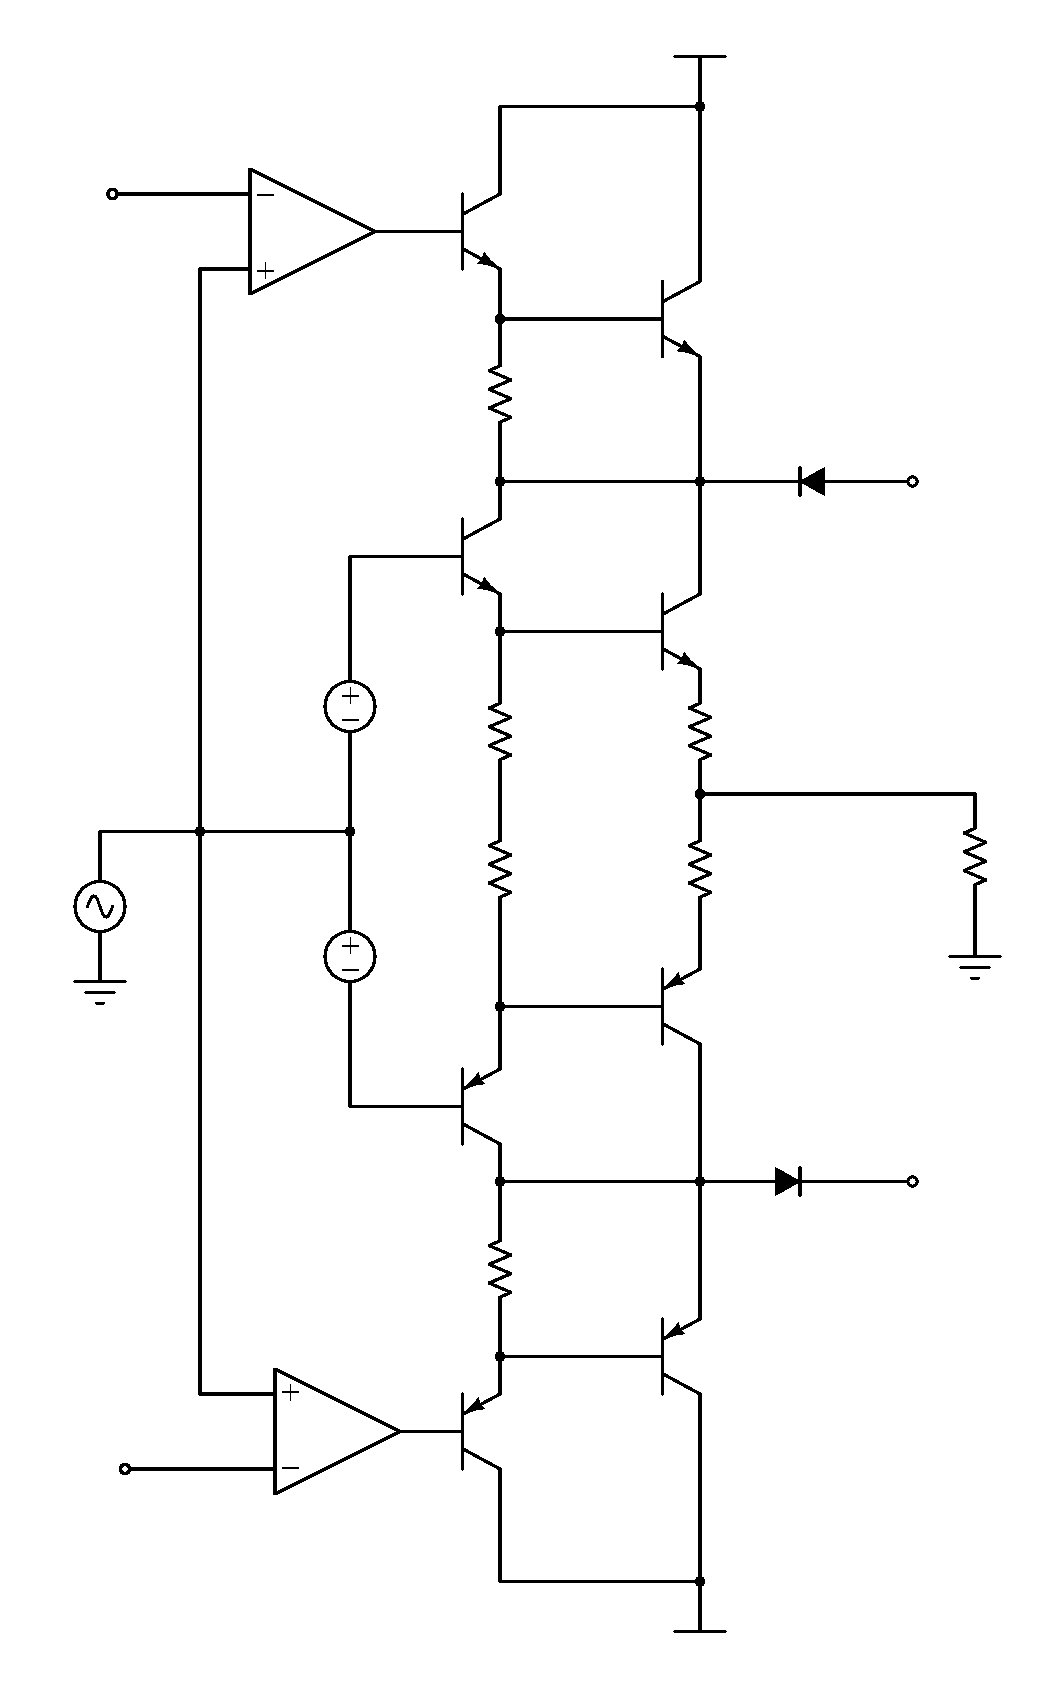
\includegraphics[scale=1]{salida}\\
   % translate x=800 y=1584 scale 0.38
   \putbox{1.39in}{6.39in}{1.20}{Vbias1}%
   \putbox{1.39in}{4.81in}{1.20}{Vbias2}%
   \putbox{5.89in}{5.39in}{1.20}{RL}%
   \putbox{4.72in}{6.22in}{1.20}{Re}%
   \putbox{4.72in}{5.31in}{1.20}{Re}%
   \putbox{4.47in}{6.89in}{1.20}{Q63}%
   \putbox{4.47in}{4.39in}{1.20}{Q64}%
   \putbox{3.14in}{7.47in}{1.20}{Q14}%
   \putbox{3.14in}{3.72in}{1.20}{Q15}%
   \putbox{3.14in}{9.56in}{1.20}{Q16}%
   \putbox{4.47in}{9.06in}{1.20}{Q62}%
   \putbox{3.14in}{1.56in}{1.20}{Q17}%
   \putbox{4.47in}{2.06in}{1.20}{Q65}%
   \putbox{0.14in}{1.31in}{1.20}{Vth-}%
   \putbox{0.06in}{9.81in}{1.20}{Vth+}%
   \putbox{4.22in}{0.06in}{1.20}{-VccH}%
   \putbox{4.22in}{10.89in}{1.20}{+VccH}%
   \putbox{6.06in}{7.89in}{1.20}{VccL+}%
   \putbox{6.06in}{3.22in}{1.20}{-VccL}%
   } % close 'parbox'
   } % close 'scalebox'
   \vspace{-\baselineskip} % this is not necessary, but looks better
}
		\caption{Etapa de salida.}
		\label{fig.salida}
	\end{figure}

	Los comparadores se encuentran conectados a la señal de entrada y a una tensión umbral Vth como referencia. Cuando la señal de entrada excede la tensión $+Vth$, el comparador (superior) hace que los transistores $Q5$ y $Q6$ se polaricen en saturación. Es decir que actúan como una llave que activa la alimentación $VccH$. A su vez el diodo $D1$ quedará polarizado en inversa ya que la tensión en el cátodo es $+VccH$, mayor que la tensión de ánodo $VccL$. Por lo tanto, el circuito queda alimentado solo mediante $+VccH$ y la potencia es manejada por dos transistores $Q6$ y $Q1$.

	De forma análoga funcionan el comparador $C2$, $Q7$, $Q8$ y $D2$ para el semicilo negativo de la señal de entrada.

	Las tensiones $Vbias1$ y $Vbias2$ permiten \textit{prepolarizar} a los transistores $Q1$ y $Q2$ con el fin de atenuar la distorsión de cruce por cero. Se deben ajustar de forma tal que la corriente de la malla de salida sea aproximadamente igual en el colector de ambos transistores ($Q1$ y $Q2$). Asimismo se debe considerar que si $ICQ$ es muy elevada se desperdicia potencia, y si es muy pequeña se obtendrá una distorsión de cruce por cero apreciable. 


\subsection{Multiplicador de $V_{BE}$}

	\begin{figure}[H]
		\centering
		\scalebox{0.5}{% XCircuit output "multiplicador.tex" for LaTeX input from multiplicador.eps
\def\putbox#1#2#3#4{\makebox[0in][l]{\makebox[#1][l]{}\raisebox{\baselineskip}[0in][0in]{\raisebox{#2}[0in][0in]{\scalebox{#3}{#4}}}}}
\def\rightbox#1{\makebox[0in][r]{#1}}
\def\centbox#1{\makebox[0in]{#1}}
\def\topbox#1{\raisebox{-0.60\baselineskip}[0in][0in]{#1}}
\def\midbox#1{\raisebox{-0.20\baselineskip}[0in][0in]{#1}}
   \scalebox{1}{
   \normalsize
   \parbox{4.18229in}{
   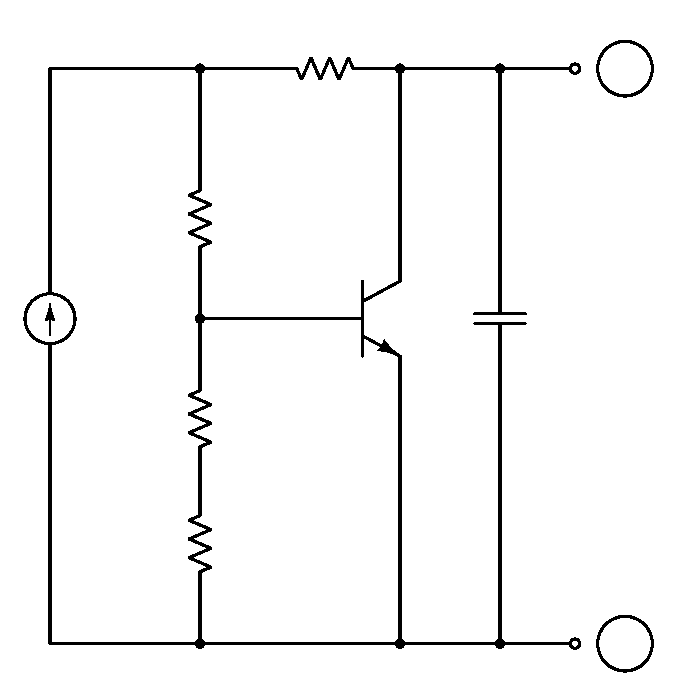
\includegraphics[scale=1]{multiplicador}\\
   % translate x=672 y=611 scale 0.38
   \putbox{3.56in}{2.32in}{1.20}{C20}%
   \putbox{2.47in}{2.32in}{1.20}{Q26}%
   \putbox{0.56in}{3.07in}{1.20}{R43}%
   \putbox{0.72in}{1.74in}{1.20}{Rp}%
   \putbox{0.64in}{0.82in}{1.20}{R44}%
   \putbox{1.89in}{4.24in}{1.20}{R42}%
   \putbox{4.06in}{4.07in}{1.20}{\centbox{\midbox{1,1}}}%
   \putbox{4.06in}{0.24in}{1.20}{\centbox{\midbox{-1,1}}}%
   \putbox{0.47in}{2.32in}{1.20}{Ipol}%
   \putbox{1.97in}{3.74in}{1.20}{$10 \Omega$}%
   \putbox{1.47in}{3.07in}{1.20}{$3,3 k\Omega$}%
   \putbox{1.39in}{0.82in}{1.20}{$680 \Omega$}%
   \putbox{1.39in}{1.65in}{1.20}{$1 k\Omega$}%
   } % close 'parbox'
   } % close 'scalebox'
   \vspace{-\baselineskip} % this is not necessary, but looks better
}
		\caption{Multiplicador de $V_{BE}$.}
		\label{fig.multiplicador}
	\end{figure}

	La resistencia $R_{3M}$ se anexa para mejorar la independencia de la tensión $V_{BE}$ con la corriente de polarización.

	\begin{equation}
		\centering
		V_M = \left( \frac{R_{1M}}{R_{1M} + R_{2M}} +1 \right) \cdot V_{BE} - I_C \cdot R_{3M} \approx  \left( \frac{R_{1M}}{R_{1M} + R_{2M}} +1 \right) \cdot V_{BE}
	\end{equation}

	 Considerando un valor de $V_{BE} \approx \SI{0.5}{\volt}$

	 \begin{equation}
	 	\centering
		\frac{\SI{2.2}{\volt}}{\SI{0.5}{\volt}} -1 = \frac{R_{1M}}{R_{2M}} \implies \boxed{R_{1M} = \num{3,4} \cdot R_{2M}}
	\end{equation}
	Se eligen los resistores comerciales $R_{1M} = \SI{3.3}{\kilo\ohm}$, $R_{2M} = \SI{680}{\ohm}$ y un potenciómetro de $\SI{1}{\kilo\ohm}$. 

\subsection{Fuente de corriente}
	El valor mínimo de la corriente necesaria para la etapa de salida se determina con el caso de máxima corriente de salida $I_{o,max} = \SI{26}{\volt}/ \SI{8}{\ohm} = \SI{3.25}{\ampere}$. Al tratarse de transistores de potencia, el factor $\beta$ es aproximadamente $\beta = 30$, por lo que la corriente de base en $Q1$ sería $I_{B,Q1} \approx \SI{110}{\milli\ampere}$. Dicha corriente es entregada por $Q_2$, siendo la corriente de base $I_{B,Q2} \approx \SI{110}{\milli\ampere}/50 \approx \SI{2}{\milli\ampere}$. A su vez la fuente polariza la etapa amplificadora de tensión (VAS), por lo que se considerará al menos el doble de dicha corriente. Se propone $I_{pol} = \SI{5}{\milli\ampere}$.

	\begin{figure}[H]
		\centering
		\scalebox{0.5}{% XCircuit output "fte.tex" for LaTeX input from fte.eps
\def\putbox#1#2#3#4{\makebox[0in][l]{\makebox[#1][l]{}\raisebox{\baselineskip}[0in][0in]{\raisebox{#2}[0in][0in]{\scalebox{#3}{#4}}}}}
\def\rightbox#1{\makebox[0in][r]{#1}}
\def\centbox#1{\makebox[0in]{#1}}
\def\topbox#1{\raisebox{-0.60\baselineskip}[0in][0in]{#1}}
\def\midbox#1{\raisebox{-0.20\baselineskip}[0in][0in]{#1}}
   \scalebox{1}{
   \normalsize
   \parbox{3.85938in}{
   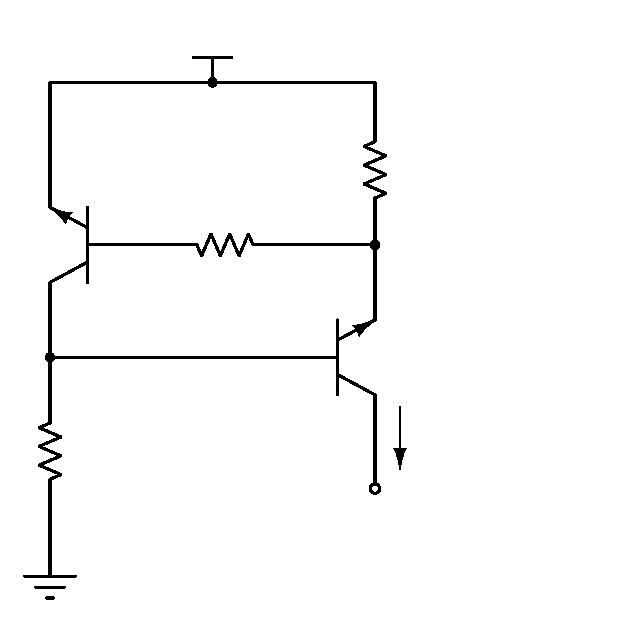
\includegraphics[scale=1]{fte}\\
   % translate x=384 y=372 scale 0.38
   \putbox{0.43in}{0.91in}{1.20}{$20 k\Omega$}%
   \putbox{2.56in}{2.83in}{1.20}{$100 \Omega$}%
   \putbox{1.47in}{2.54in}{1.20}{$2,2 k\Omega$}%
   \putbox{2.76in}{1.16in}{1.20}{$5 mA$}%
   \putbox{0.97in}{3.74in}{1.20}{VccH+}%
   \putbox{1.97in}{2.87in}{1.20}{R1}%
   \putbox{1.01in}{2.54in}{1.20}{R2}%
   \putbox{2.81in}{0.83in}{1.20}{$I_{pol}$}%
   \putbox{0.51in}{2.87in}{1.20}{$V_{BE}$}%
   \putbox{1.18in}{1.83in}{1.20}{$V_{BE}$}%
   \putbox{0.72in}{2.16in}{1.20}{\textcolor{blue}{$30V-V_{BE}$}}%
   } % close 'parbox'
   } % close 'scalebox'
   \vspace{-\baselineskip} % this is not necessary, but looks better
}
		\caption{Fuente de corriente.}
		\label{fig.fte}
	\end{figure}



\subsection{Comparadores}

	\begin{figure}[H]
		\centering
		\scalebox{0.5}{% XCircuit output "comparador.tex" for LaTeX input from comparador.eps
\def\putbox#1#2#3#4{\makebox[0in][l]{\makebox[#1][l]{}\raisebox{\baselineskip}[0in][0in]{\raisebox{#2}[0in][0in]{\scalebox{#3}{#4}}}}}
\def\rightbox#1{\makebox[0in][r]{#1}}
\def\centbox#1{\makebox[0in]{#1}}
\def\topbox#1{\raisebox{-0.60\baselineskip}[0in][0in]{#1}}
\def\midbox#1{\raisebox{-0.20\baselineskip}[0in][0in]{#1}}
   \scalebox{1}{
   \normalsize
   \parbox{7.08333in}{
   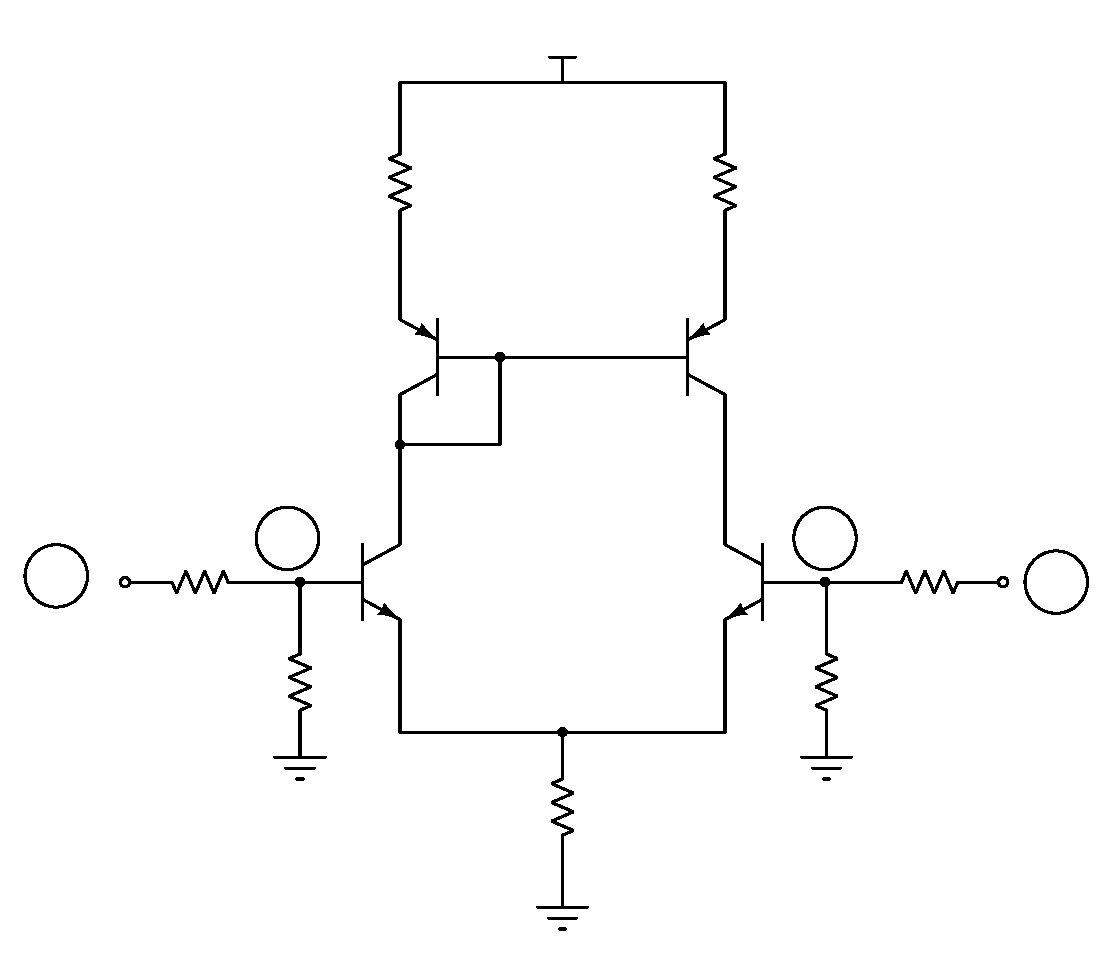
\includegraphics[scale=1]{comparador}\\
   % translate x=928 y=636 scale 0.38
   \putbox{2.58in}{2.33in}{1.20}{Q9}%
   \putbox{4.45in}{2.29in}{1.20}{Q10}%
   \putbox{2.37in}{3.81in}{1.20}{Q11}%
   \putbox{4.66in}{3.81in}{1.20}{Q12}%
   \putbox{3.35in}{5.95in}{1.20}{+VccH}%
   \putbox{0.14in}{2.33in}{1.20}{Vo}%
   \putbox{3.18in}{0.83in}{1.20}{Rec}%
   \putbox{1.10in}{2.54in}{1.20}{R1}%
   \putbox{1.47in}{1.70in}{1.20}{R2}%
   \putbox{5.97in}{2.49in}{1.20}{R3}%
   \putbox{5.01in}{1.66in}{1.20}{R4}%
   \putbox{2.18in}{5.04in}{1.20}{R5}%
   \putbox{4.35in}{4.99in}{1.20}{R6}%
   \putbox{1.64in}{2.58in}{1.20}{Vo'}%
   \putbox{5.18in}{2.58in}{1.20}{Vth'}%
   \putbox{6.76in}{2.33in}{1.20}{Vth}%
   \putbox{2.76in}{5.04in}{1.20}{56}%
   \putbox{4.93in}{5.04in}{1.20}{56}%
   \putbox{1.10in}{2.08in}{1.20}{5,6k}%
   \putbox{2.06in}{1.70in}{1.20}{1k}%
   \putbox{5.51in}{1.70in}{1.20}{1k}%
   \putbox{5.89in}{2.08in}{1.20}{8,2k}%
   \putbox{3.81in}{0.83in}{1.20}{560}%
   } % close 'parbox'
   } % close 'scalebox'
   \vspace{-\baselineskip} % this is not necessary, but looks better
}
		\caption{Comparador.}
		\label{fig.comparador}
	\end{figure}

	Se propone la configuración de par diferencial de la figura para implementar los comparadores. Se utiliza una fuente de corriente espejo para lograr mayor estabilidad. En vez de comparar con la señal proveniente de la etapa VAS, se compara con la señal de salida $V_{o}$ para evitar cargar la VAS con la resistencia de entrada que presenta el par diferencial ($2\cdot r_\pi$). La señal de salida no resulta alterada por tratarse de un colector común que es separador de impedancias.
	Por otra parte, es difícil lograr en la práctica que los transistores que conforman el par diferencial manejen una excursión de tensión de hasta \SI{30}{\volt}, por lo que se utiliza un divisor resistivo en ambas bases de los transistores para atenuar la amplitud de tensión. Es conveniente que la tensión de referencia $Vth'$ sea levemente menor que la prevista con el fin de contrarrestar el retardo de tiempo del comparador.

\begin{equation}
	\centering
	V_{th}' = V_{th} \cdot \frac{R_4}{R_4 + R_3} \implies \SI{1.5}{\volt} = \SI{12}{\volt} \cdot \frac{R_4}{R_4 + R_3} \implies \boxed{R_3 = 7 \cdot R_4}
\end{equation}

\begin{equation}
	\centering
	V_o' = V_o \cdot \frac{R_2}{R_2 + R_1} \implies \SI{2}{\volt} = \SI{12}{\volt} \cdot \frac{R_2}{R_2 + R_1} \implies \boxed{R_1 = 5 \cdot R_2}
	\end{equation}

	El valor de la resistencia de emisor $R_{ec}$ se elige en función de la máxima tensión posible en $V_o$ y la corriente que circularía en reposo. Con $R_ec = \SI{500}{\ohm}$ se obtiene:

	\begin{equation}
		\centering
		I_{e,max} = \frac{ \SI{1.3}{\volt} }{ \SI{500}{\ohm} } = \SI{2.6}{\milli\ampere}
	\end{equation}

	\begin{equation}
		I_{e,pol} = \frac{ \SI{0.8}{\volt} }{ \SI{500}{\ohm} } = \SI{1.6}{\milli\ampere} \implies \SI{1.28}{\milli\watt}
	\end{equation}

